\section{Evaluation}
\label{sec:results}
\subsection{Envelope extraction evaluation}
\label{sec:offline_tests}
%
\begin{figure*}[t!]
\centering
\subfigure[] {
        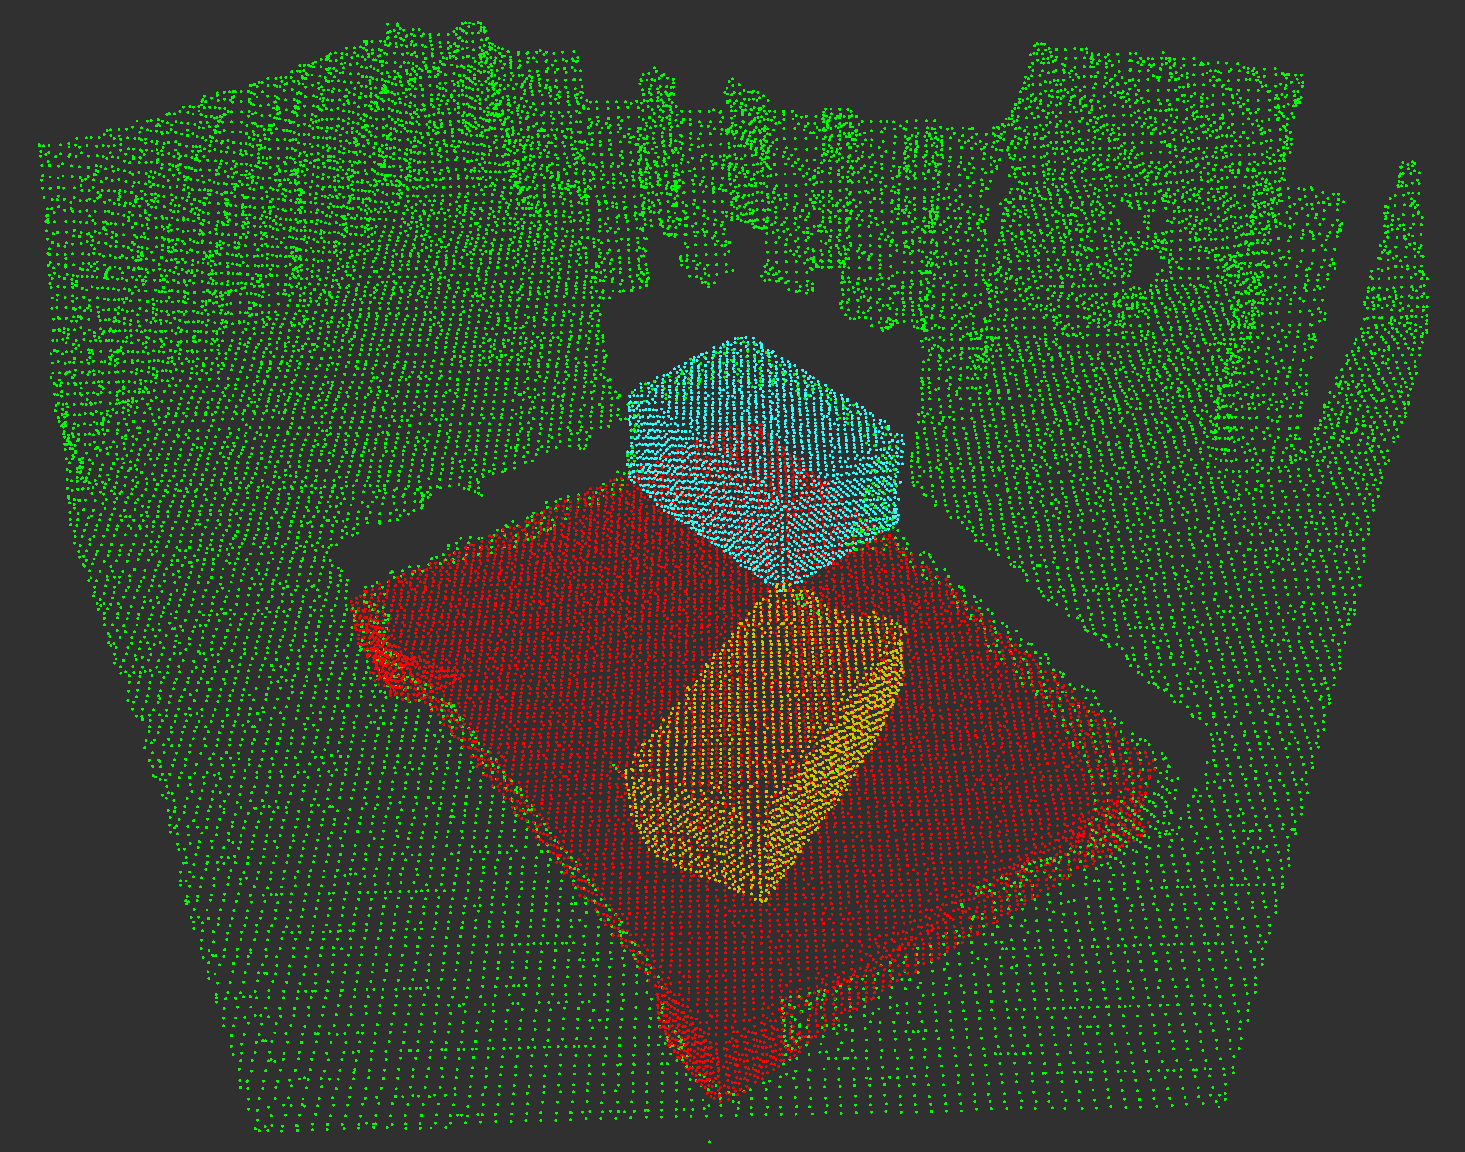
\includegraphics[width = 0.46\linewidth, height=6.0cm]{figs/shelves}
	\label{fig:shelves}
}
\subfigure[] {
        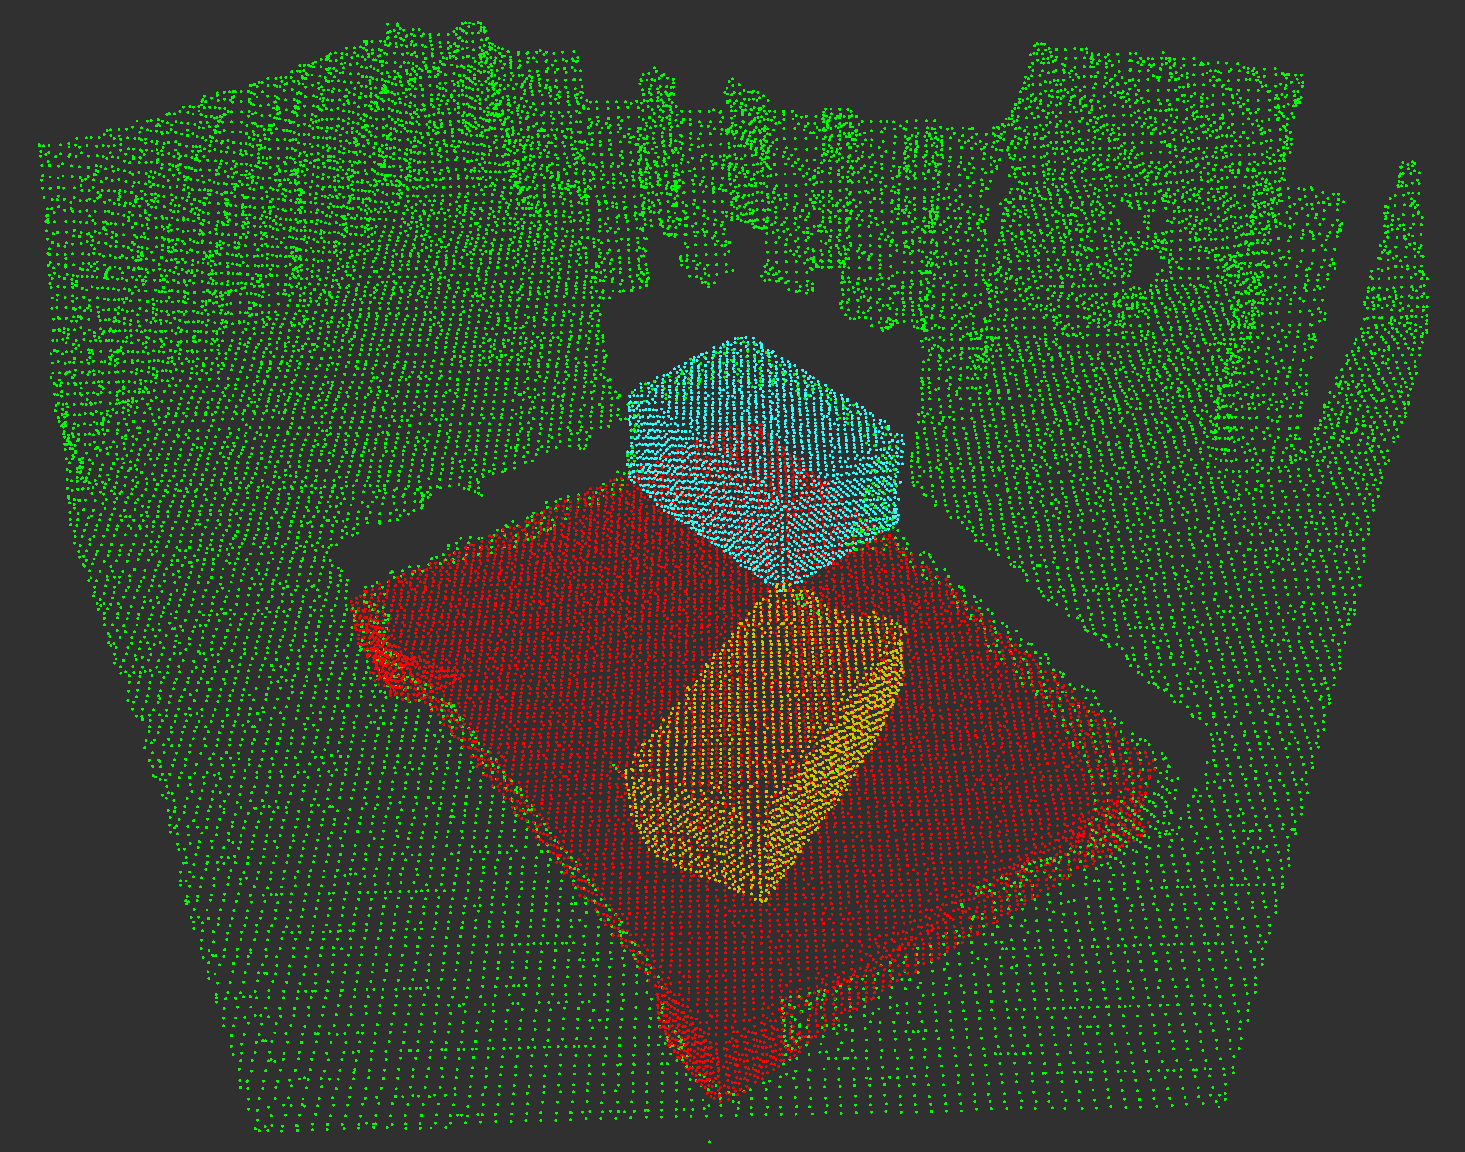
\includegraphics[width = 0.46\linewidth, height=6.0cm]{figs/tables}
	\label{fig:tables}
}
\caption{Illustration of the test environments used in this paper: \subref{fig:shelves} shows the TSDF models of the five scenes from the \textit{shelves} data set, reconstructed at $5$~mm resolution; \subref{fig:tables} shows the models of the \textit{table} data set at $10$~mm resolution.}
\label{fig:environments}
\end{figure*}
%
%\begin{figure}[t!]
%\centering
%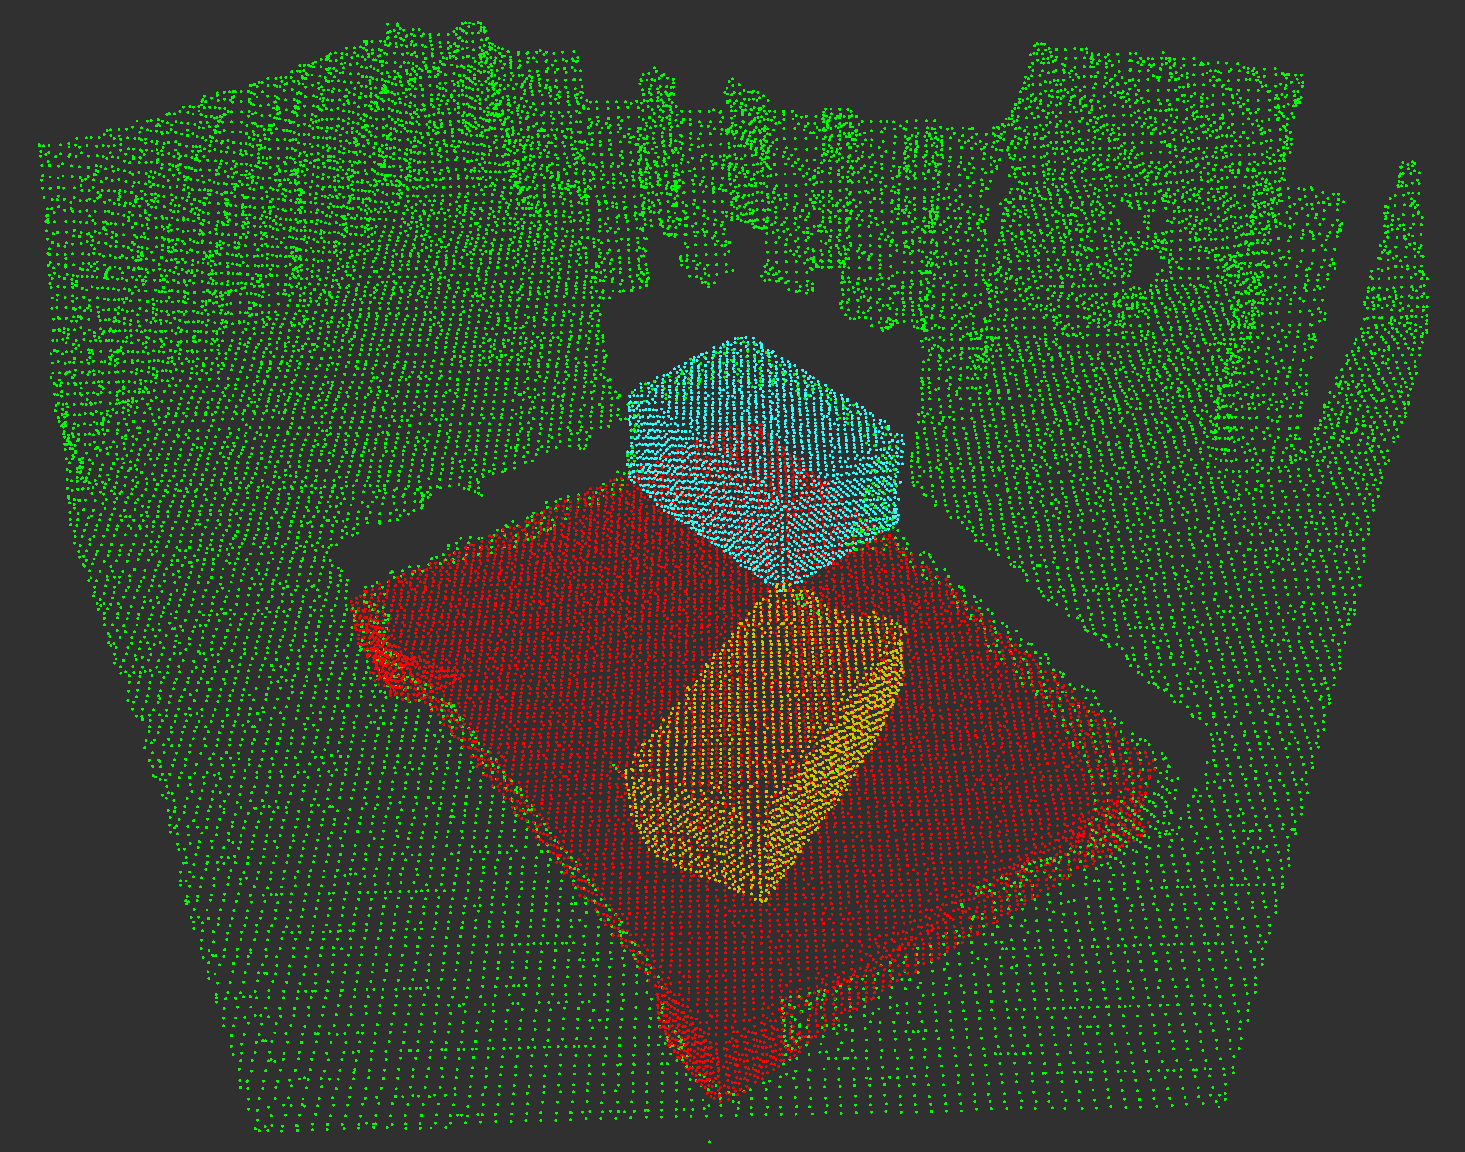
\includegraphics[width = .9\linewidth]{figs/objects}
%\caption{The five test objects used in the evaluation. The two plush toys were evaluated with spherical envelope primitives fit to the head, while the remaining objects were associated with cylindrical primitives.}
%Cup\label{fig:objects}
%\end{figure}
As a first step, we evaluated the proposed grasp envelope fitting approach on a set of five test
objects placed in ten different scenes. Here, the purpose was to evaluate the computational effort
of the envelope extraction procedure, as well as the quality of the obtained envelopes. Under the assumption
that all grasps which respect the envelope constraints are successful, envelope quality $Q$ is
defined as the number of valid gripper pose samples from $S$ that fall within the grasp envelope. This measure
directly relates to the enclosed volume of the envelope constraints. Thus, envelopes with larger
quality $Q$ allow for more gripper pre-grasp posture redundancy and easier grasp acquisition. Two plush toys (a teddy bear and a pig), a water bottle, a large cup and a cardboard box (shown in
Fig.~\ref{fig:objects}), all graspable by the considered gripping device, were chosen as target objects.
We placed the objects in different poses in two different types of scenes, models of which are shown in Fig.~\ref{fig:environments}. 
For the first set of five scenes, the objects were placed on shelves in an office environment, resulting in a moderately cluttered setup.
Conversely, in the second set, objects were placed on a table top and were spaced further apart from each other.
These two sets of environments (referred to as the \textit{shelves} and \textit{table} data sets) were scanned using a hand-held Asus Xtion Pro\footnote{\url{http://www.asus.com/Multimedia/Xtion_PRO_LIVE/}} RGB-D camera.
The sensor pose was tracked using the SDF Tracker algorithm~\cite{Cane13a}.
The shelves data set was reconstructed at grid resolutions of $5$~mm and $10$~mm, while the table data set was reconstructed only at a resolution of $10$~mm, as the lower number of geometrical features in the latter caused bad tracker performance at higher grid resolutions.
Object poses and bounding sphere/cylinder size were manually determined for each test case.
\par
We pre-computed two sets of spherical and cylindrical grasp envelopes, using collision grid resolutions of $5$~mm and $10$~mm respectively.
For the cylindrical envelopes, we sampled poses at $15$ radial distances with $0.1$~m $\leq d \leq 0.3$~m, $100$ orientations with $0\leq \alpha \leq 2\pi$~rad and $7$ vertical slices over a span of $0.2$~m.
The spherical primitive was sampled at $15$ distances $r$ and $100$ orientations, using the same metric bounds, as well as $7$ different inclinations.
In both cases, this resulted in a 3D sampling grid $\mathcal{S}$ of $10500$ gripper poses.
A visual example of the results obtained for the extracted grasp envelope of one of the objects in the shelves data set is shown in Fig.~\ref{fig:example}.
%\begin{figure}[t!]
%\centering
%\includegraphics[width = \linewidth]{figs/grasp_illustration_v2}
%\caption{Illustration of the test environments used in this paper: \subref{fig:example}}
%\label{fig:example}
%\end{figure}
\par
In addition to visual inspection, we also measured for each grasp envelope the computation time
spent in extracting it and the quality metric $Q$. Fig.~\ref{fig:result} shows a boxplot of the
obtained envelope qualities per object and data set, with each box centered on the mean and spanning
the area between the $25$th and $75$th percentile. We can draw several conclusions from the results
shown in Fig.~\ref{fig:result}. First, it is evident that the less cluttered table data set results
in substantially larger grasp envelopes, validating that the proposed method is able to find grasp
envelopes with higher quality for objects that are easier to grasp.
Second, by comparing results on the two reconstructions of the shelves data set, we note that the grasp envelopes extracted from higher resolution models are slightly larger.
This effect is due to the more precise collision checks performed.
However, in our tests the performance gain by using a higher resolution does not seem significant, most likely owing to the fact that the amount of clutter in the scenes is not extremely high.
As this performance gain comes at a price of an order of magnitude slower computational time, we conclude that very precise environment models should only be utilized when necessary.
Finally, we note that the performance of the proposed method is worst for the cup object. 
Upon further investigation, this artifact can be explained by a particularity of the TSDF representation used to model the environment: it is particularly susceptible to modeling errors on thin objects observed from multiple viewpoints. 
As both the outer and inner walls of the cup are often visible in our data sets, the fidelity of the models is often not optimal, resulting in lower certainty on the extracted grasp envelopes.
Regarding computational performance, our approach extracts grasp envelopes in roughly $200$~ms at a resolution of $5$~mm and  $20-40$~ms at a $10$~mm resolution (using a single core of an Intel Xeon CPU E5-1620 v3 at 3.50GHz).
Most of the time is spent on computing the valid samples as per Sec.~\ref{sec:collision_check}, with only a small fraction of resources expended on extracting the maximum volume envelope.
%
\begin{figure*}[t!]
\centering
\subfigure[] {
        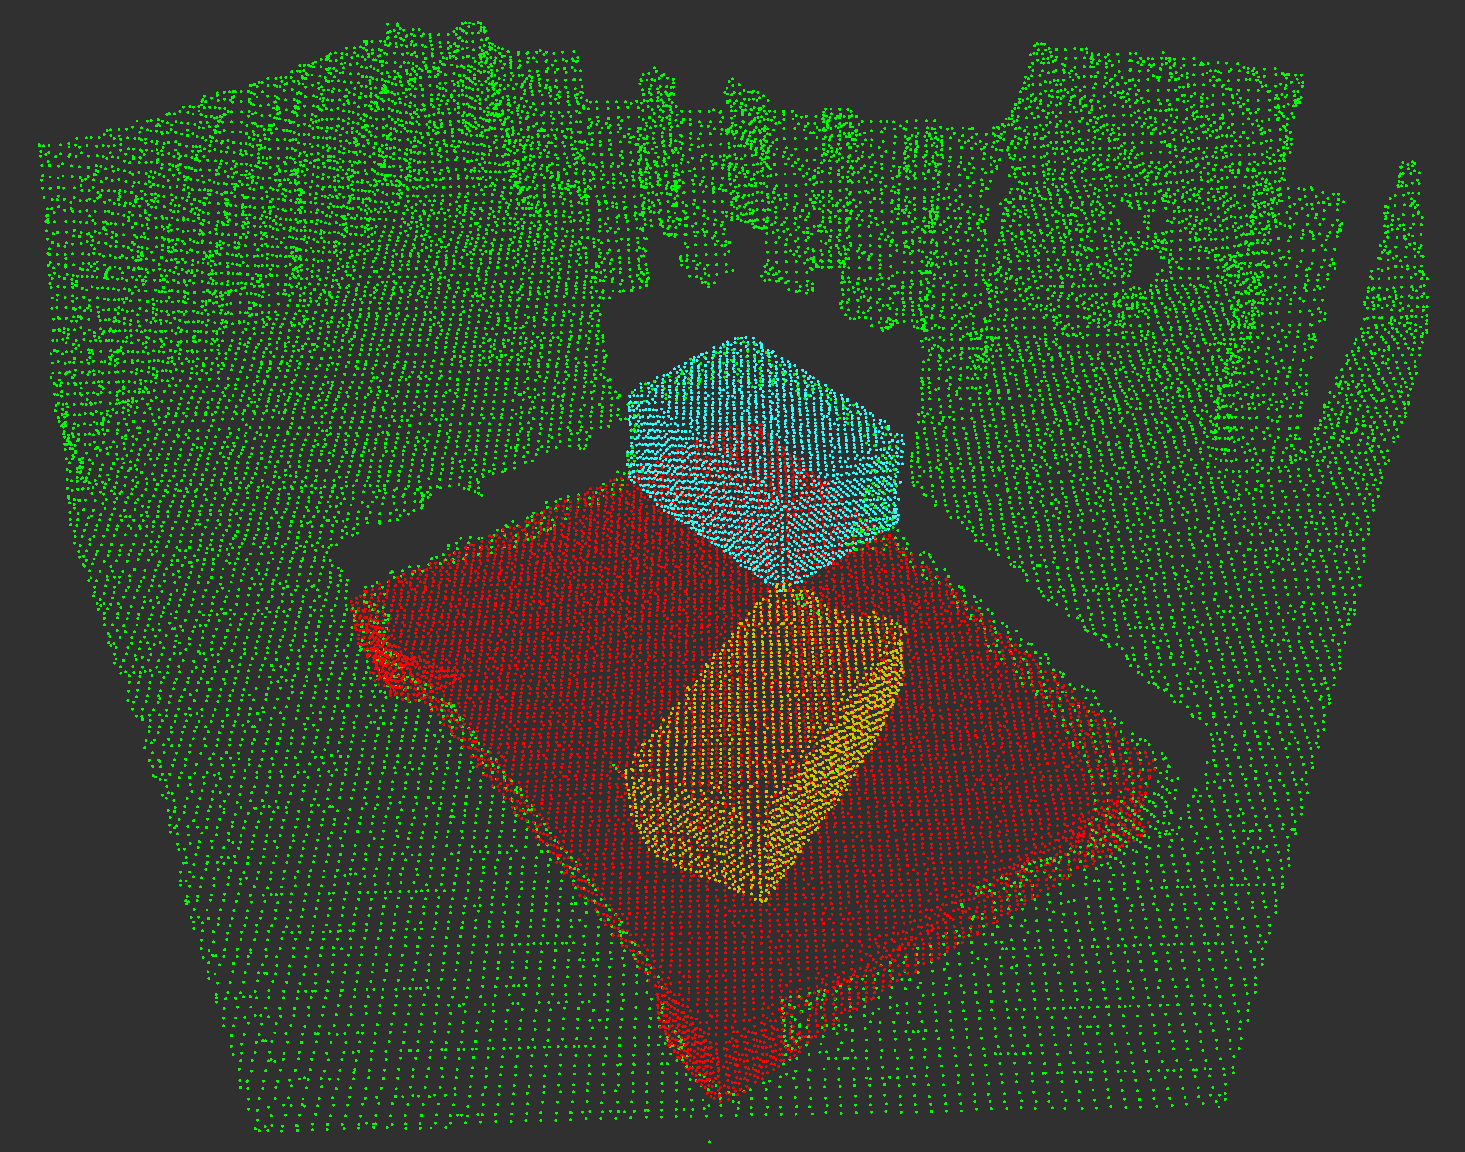
\includegraphics[width = 0.3\linewidth, height=5.0cm]{figs/objects}
	\label{fig:objects}
}
\subfigure[] {
        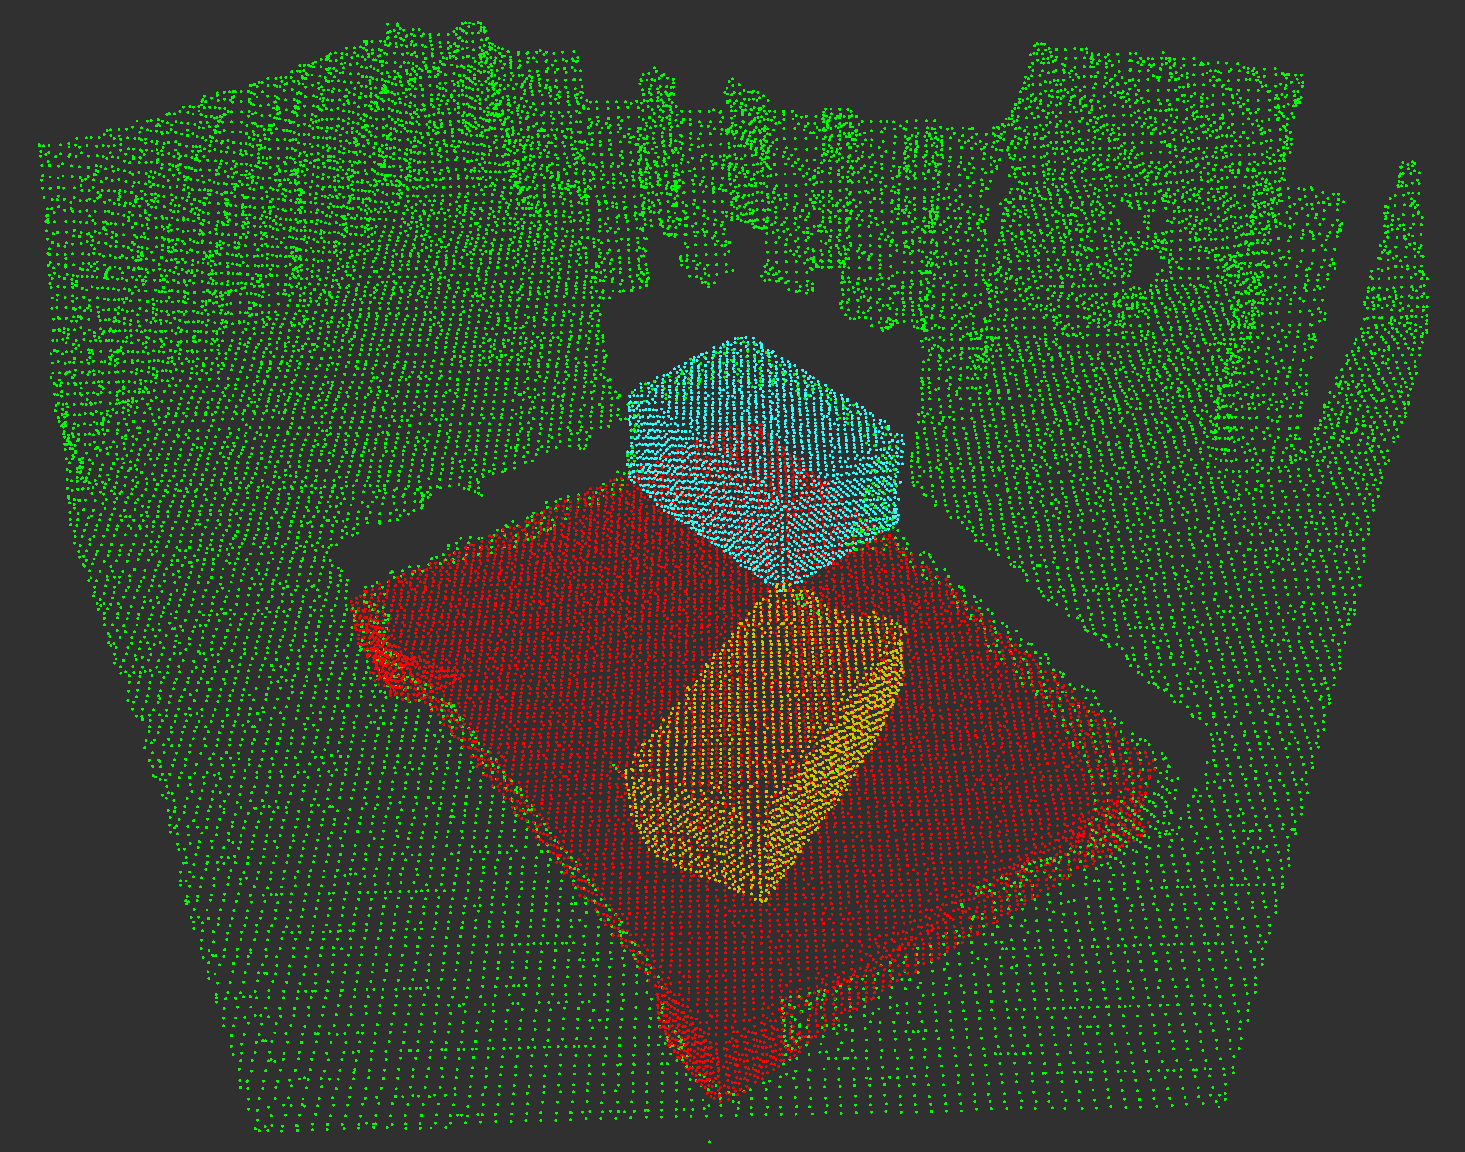
\includegraphics[width = 0.3\linewidth, height=5.0cm]{figs/grasp_illustration_raster}
	\label{fig:example}
}
\subfigure[] {
        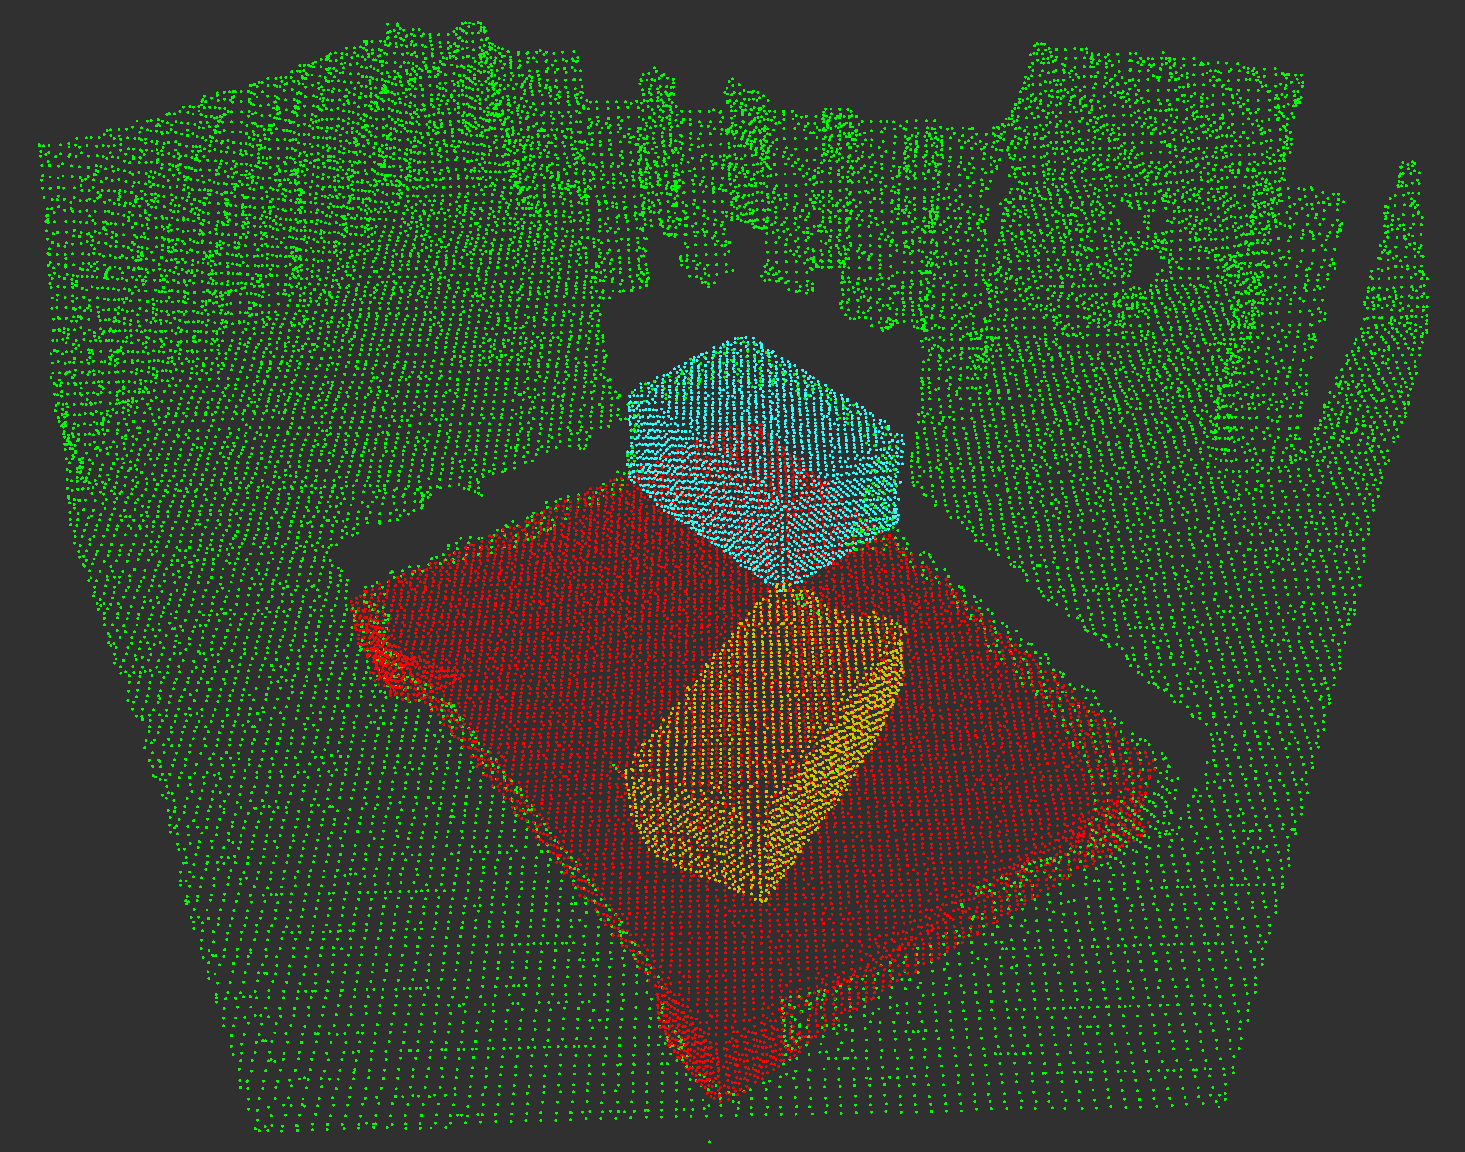
\includegraphics[width = 0.3\linewidth, height=5.0cm]{figs/results}
	\label{fig:result}
}
\caption{\subref{fig:objects} shows the five test objects used in the evaluation. The two plush toys were evaluated with spherical envelope primitives fit to the head, while the remaining objects were associated with cylindrical primitives. \subref{fig:example} illustrates typical constraint envelopes extracted for objects in cluttered environments; \subref{fig:result} summarizes results of the proposed grasp envelope extraction method, showing the distribution of envelope quality $Q$ over different objects and scenes. }
\label{fig:results}
\end{figure*}
%
\subsection{Grasp acquisition success evaluation}
\label{sec:online_evaluation}
%
\begin{figure*}[t!]
\centering
\subfigure[] {
        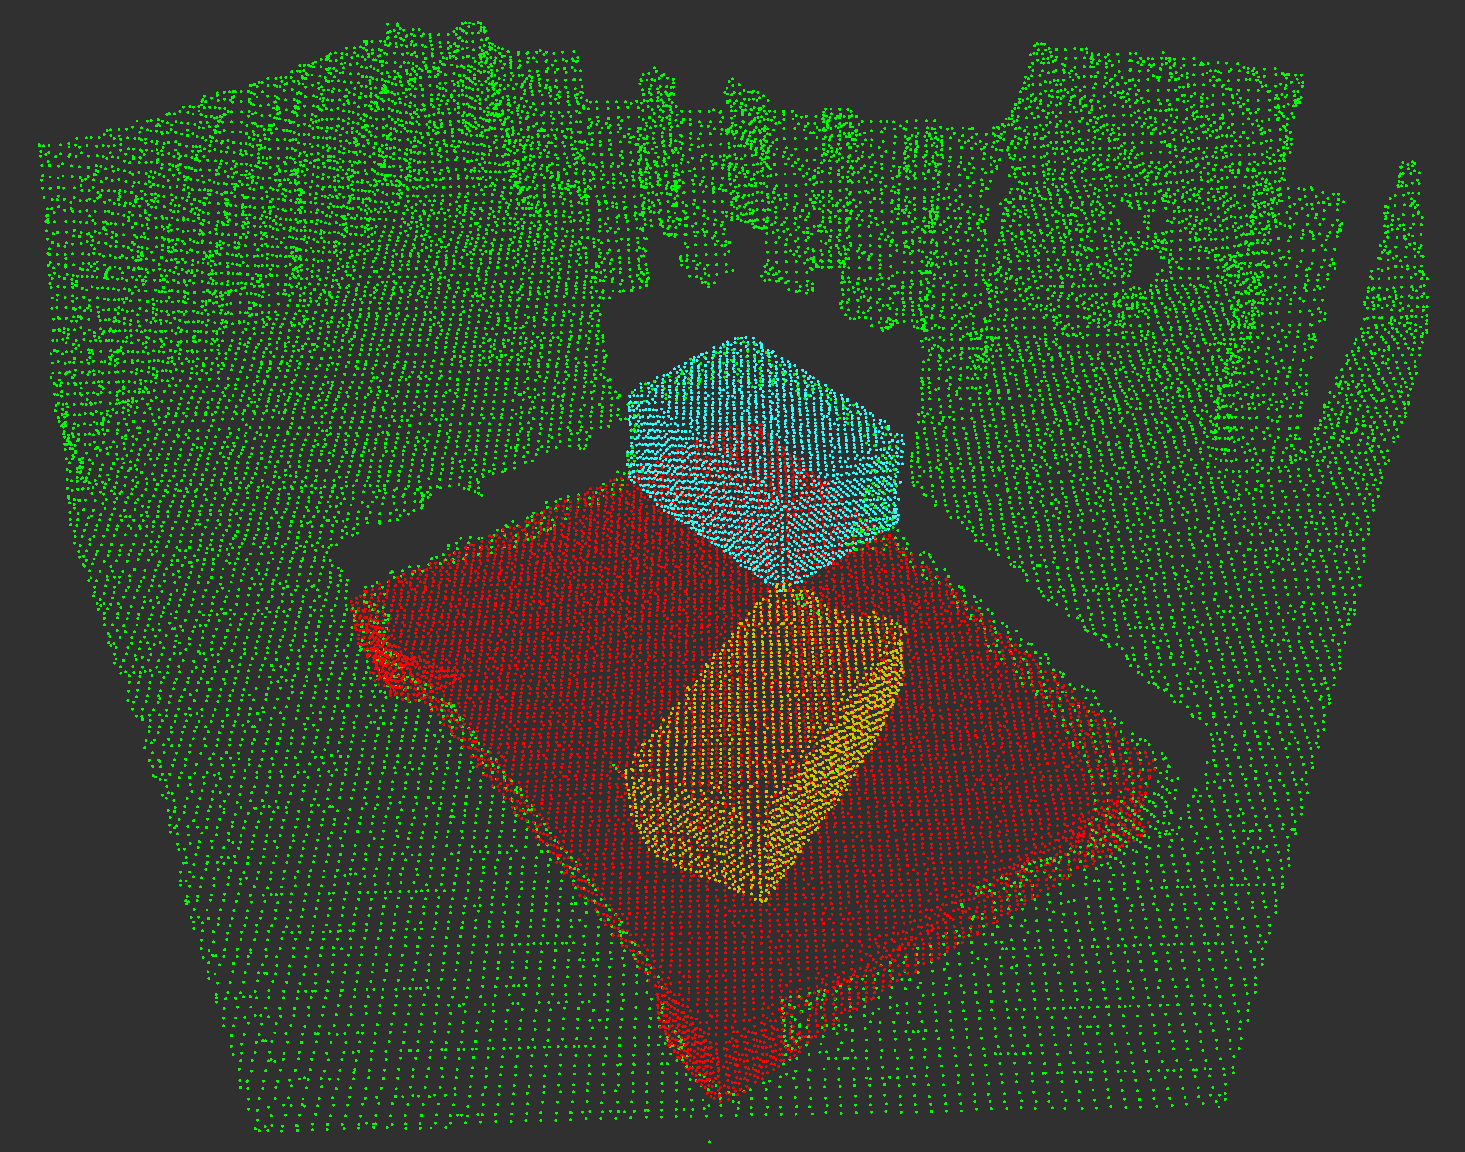
\includegraphics[width = 0.46\linewidth, height=5.0cm]{figs/sample_scene2}
	\label{fig:sample_run}
}
\subfigure[] {
        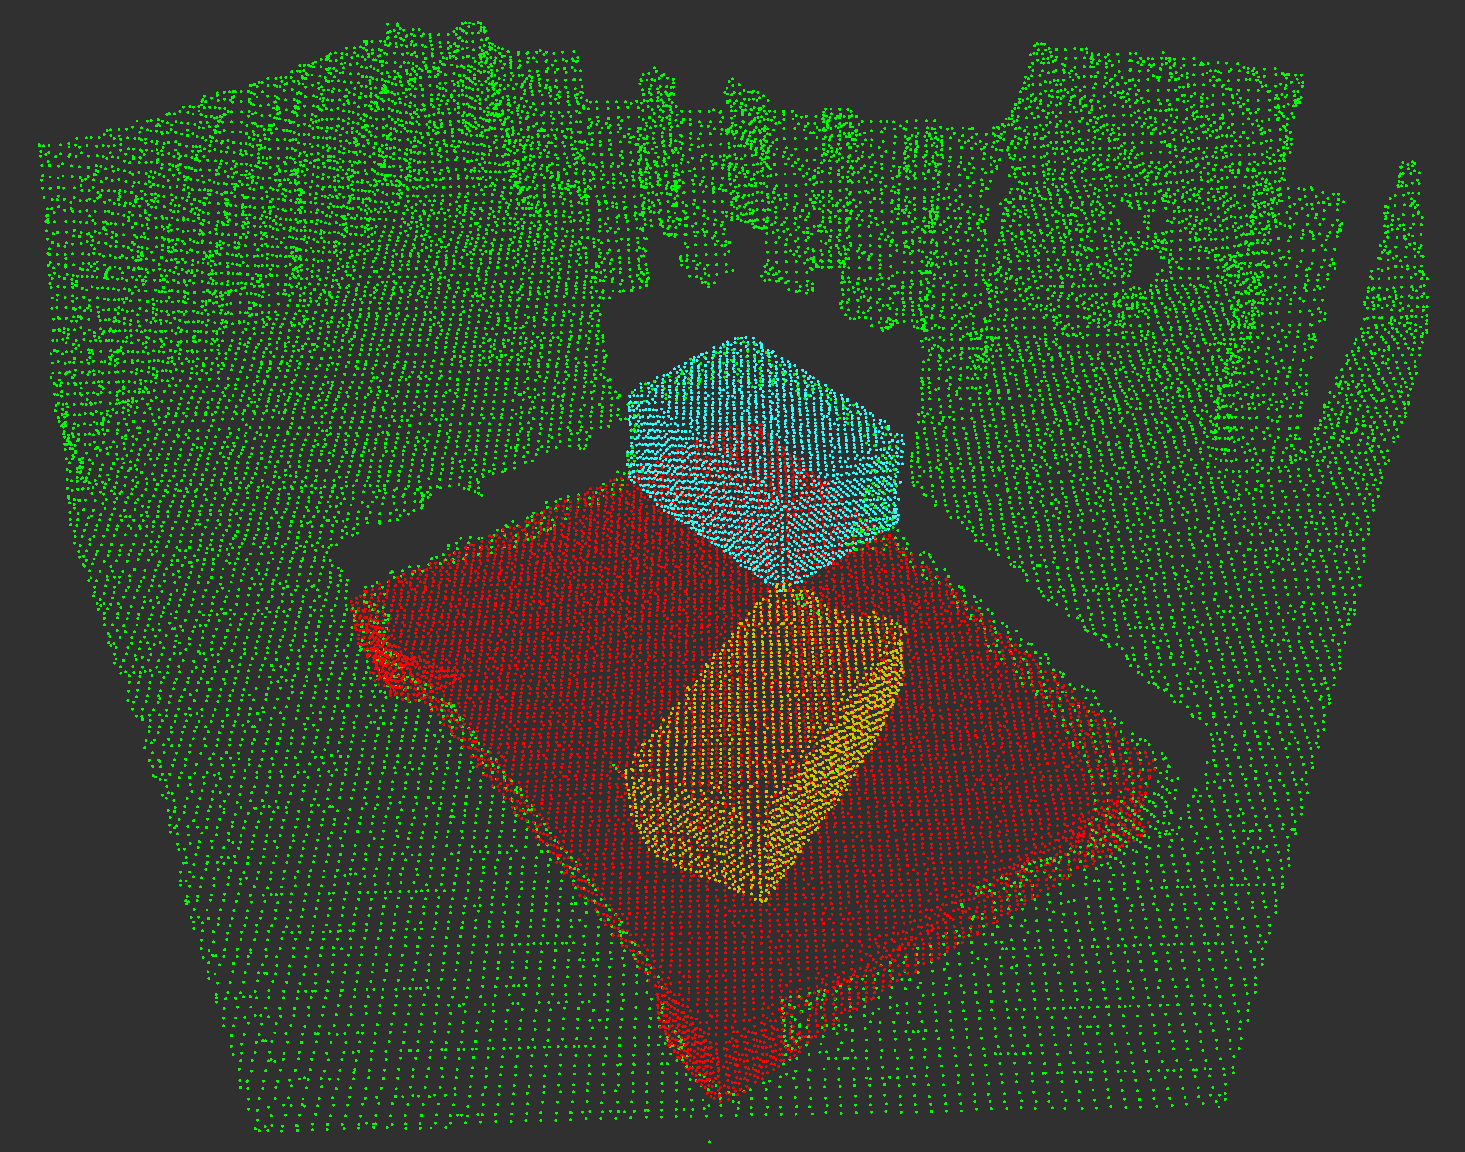
\includegraphics[width = 0.46\linewidth, height=5.0cm]{figs/sample_experiment}
	\label{fig:sample_run_rviz}
}
\caption{Setup used for the experiments in Sec.~\ref{sec:online_evaluation}. A sample scene used in the evaluation is shown in~\subref{fig:sample_run}. A reconstructed test scene model and a corresponding grasp envelope (visualized as a set of selected grasping configurations) are shown in~\subref{fig:sample_run_rviz}.}
\label{fig:tests2}
\end{figure*}
%
%
\renewcommand{\arraystretch}{1.5}
\renewcommand{\tabcolsep}{1.5mm}
\begin{table*}[t!h]
  \caption{Grasp Acquisition Evaluation}
  \vspace{-0.45cm}
  \begin{center}
    \begin{tabular}{l|c|c|c|c|c|c|c|c|c|c}
      Object  & \# of exp. & Success & Rate [\%] & $Q$ & $l \, [rad]$ & $t^p \, [s]$ & $t^e \, [s]$ & $t^m \, [s]$ & $t^g \, [s]$  & $\sum t \, [s]$     \\
      \hline \\ [-3.2ex]
      Duplo  & $20$ & $17$ & $85.0$ & $161.4\pm109.4$ & $4.3 \pm 0.9$ & $14.9 \pm 3.0$ & $0.06 \pm 0.11$ & $25.9 \pm
      3.8$ & $14.7 \pm 3.9$ & $55.6 \pm 5.3$ \\
      Cup    & $16$ & $16$ & $100.0$ & $51.2\pm27.5$ & $4.7 \pm 1.3$ & $13.7 \pm 3.5$ & $0.06 \pm 0.05$ & $10.8 \pm
      0.2$ & $6.9 \pm 2.6$ & $31.5 \pm 3.7$ \\
      Bottle & $17$ & $15$ & $88.2$ & $67.1\pm68.3$ & $4.9 \pm 2.3$ & $14.0 \pm 3.3$ & $0.03 \pm 0.05$ & $10.8 \pm
      0.4$ & $8.5 \pm 3.9$ & $33.3 \pm 6.1$ \\
      Ball   & $20$ & $17$ & $85.0$ & $32.7\pm16.6$ & $5.6 \pm 0.4$ & $13.9 \pm 3.4$ & $0.06 \pm 0.05$ & $10.8 \pm
      1.4$ & $13.9 \pm 4.3$ & $38.7 \pm 4.9$ \\
      Teddy  & $19$ & $12$ & $63.2$ & $28.9\pm13.8$& $5.6 \pm 0.5$ & $15.5 \pm 2.8$ & $0.06 \pm 0.07$ & $10.6 \pm
      0.9$& $11.5 \pm 4.6$ & $37.8 \pm 4.3$ \\
      \hline
      Total & $92$ & $77$ & $83.7$ & $69.46\pm78.06$ & $5.0 \pm 1.3$ & $14.4 \pm 3.2$ & $0.06 \pm 0.07$ & $14.1 \pm
      6.6$ & $11.4 \pm 4.9$ & $39.9 \pm 10.0$\\
    \end{tabular}
    \label{tab:grasp_acquisition}
  \end{center}
 \vspace{-0.25cm}
\end{table*}
%
%
In order to evaluate the usefulness of the extracted envelopes for the purpose of autonomous grasp
acquisition, we also integrated the proposed envelope extraction algorithm into the inequality
Stack-of-Tasks (SoT)~\cite{Kano11} manipulator control framework implementation we presented in~\cite{Krug15}. 
In our experimental setup, we mounted the Velvet Fingers gripper (augmented with an Asus Xtion Pro depth camera) on a KUKA LWR 4+ robot. 
We roughly (by hand) placed one of the target objects shown in Fig.~\ref{fig:setup} at a known picking location, while the other four objects were placed pseudo-randomly in the workspace to simulate clutter (sample scene configuration shown in Fig.~\ref{fig:sample_run}).
The five objects used in these experiments were: a plush teddy bear (Teddy, $82$ g), a stack of
duplo blocks (Duplo, $60$ g), a water bottle (Bottle, $103$ g), a coffee mug (Cup, $134$ g), and a
toy ball (Ball, $54$ g). The two grasp envelope primitives generated in the previous sub-section (at a model resolution of $10$~mm) were used also in this trial: the cylindrical primitive was associated to the Bottle, Cup and Duplo objects, while the spherical one was used for the Teddy and Ball objects. 
%
\par
In each experimental run we first controlled the manipulator to move the gripper-mounted camera to three pre-defined scene observation poses.
Simultaneously we built a TSDF model from the depth images, using camera poses obtained through the robot's forward kinematic model. 
We then used our grasp envelope extraction procedure to obtain constraints on the gripper posture
for the target object, which were subsequently used to form control tasks used in the SoT framework (see~\cite{Krug15} for a more in-depth description).
At this point, we made a slight modification to the envelope extraction procedure in order to obtain
envelopes that were more likely to be reachable for the employed robot arm. 
To this end, we imposed additional constraints on the gripper orientation prior to extracting the
grasping envelopes, requiring the final end effector orientation to be within a cone of width $\frac{\pi}{2}$~rad, centered at the initial end effector orientation.
A sample grasp envelope extracted in this manner from a training scene is shown in Fig.~\ref{fig:sample_run_rviz}.
Once the manipulator motion control satisfied the grasp envelope constraints, we executed the grasp
acquisition routine described in~\cite{Krug14a}, in order to obtain an enveloping grasp of the target object.
A trial was judged successful if the target object could be lifted and extracted from the scene. 
We performed twenty trials for each target object, with varying placement poses of the surrounding objects in the scene.
\par
The results of this set of experiments are summarized in Table~\ref{tab:grasp_acquisition}.
For each of the test objects we report respectively: 
the number of experiments performed; 
the number of successful grasps; 
the respective success rate; 
the grasp envelope quality $Q$; 
the trajectory length $l=\int_0^{t^m}\norm{\dot{\mbm{q}}(t)}_1dt$ as the sum of angular distances traveled by all joints of the manipulator; 
the times $t^p$, $t^e$, $t^m$, and $t^g$ for the pre-positioning, envelope extraction, grasp pose
approach motion and grasp acquisition phases respectively; 
as well as the total time for each run $\sum t$.  
In eight of the trials the target object was occluded from the sensor view point and our approach did not find a suitable grasping envelope. 
These trials are excluded from the statistics in Table~\ref{tab:grasp_acquisition}.
\par
The obtained statistics are relatively uniform across the different trials and different objects, with two minor exceptions.
First, the success rates for the Teddy are notably lower than for the rest of the target objects.
This discrepancy is unlikely to be linked to the size of the extracted envelopes, which are almost on par with the other object associated to a spherical envelope primitive (the Ball).
We attribute the lower success rate chiefly to the lower friction coefficient of the Teddy, which leads to frequent slippage against the belts of the Velvet Fingers gripper and consequently a lower likelihood of attaining a stable grasp. 
The second discrepancy is in the substantially longer trajectory execution times ($t^m$) for the Duplo object. 
The reason for this is that the underlying task dynamics parameters in the SoT framework were adjusted after the tests on the Duplo object, in order to speed up testing.
We also note the reasons for failure in grasping for the remaining objects: for the Duplo object, two failures were due to the object toppling over and one failure was due to a collision with an obstacle during approach; for the Bottle, both failures were due to the object toppling; finally, for the Ball all three failures were due to the object rolling out of the gripper upon contact. 
Finally, the grasp envelope extraction procedure produced slightly smaller volumes in comparison to the offline tests from Sec.~\ref{sec:offline_tests}, due to the additional constraint on end effector orientation. 
The reported envelope extraction run-times $t^e$ were consistent, allowing for some overhead for message passing between different nodes.
%
